\section{Discussion}
\label{sec:discussion}


\subsection{Feed-Forward Neural Network} Both feed-forward networks
achieved good accuracy on the validation set. The multiple hidden
layer architecure was able to perform better than its single layer
counter part. This could be because of the deeper layers learning more
complex relationships between the tokens in the tweet, as the single
hidden layer was learning patterns of spam tweets.

\subsection{Long Short-Term Memory }
The assumption was that LSTM would achieve a batter accuracy, but it did not. In our problem the single hidden layer feed forward network achieved a better accuracy. However, we couldn’t tell if the difference in the accuracy because of the model choice or the embedding approach since we used different approach for each model. Therefore, we tried to use the same model architecture that we used in the multiple hidden layered feed-forward neural network approach with this pre-trained GloVE embedding. The results was worse than LSTM with accuracy for testing data: 79\% and in the validation data: 83\% Figure \ref{fig:nnpre}
 \begin{figure}[h!]
  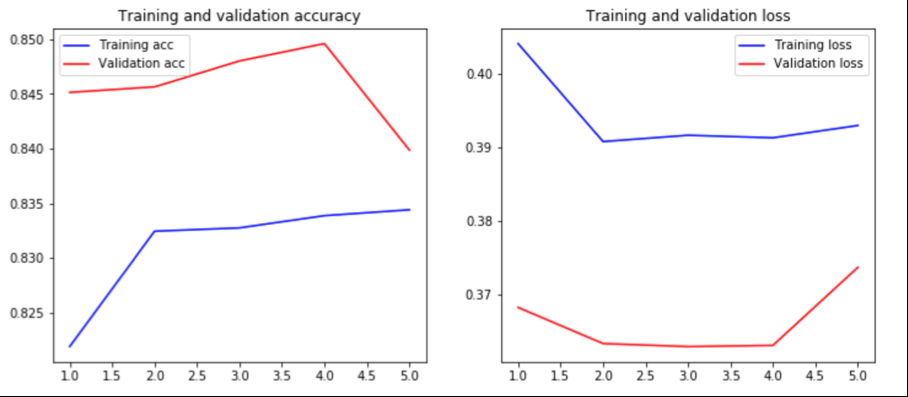
\includegraphics{nnPretrain.png}
  \caption{multiple hidden layered feed-forward neural network approach with pre-trained GloVE embedding.}
  \label{fig:nnpre}
\end{figure} . 
\\ One of the future work that can be done here is to do the same LSTM model with word embedding that are trained in our data instead of using the pre trained Glove to test the other hypothesis that embedding by training on our tweets is the reason of the better accuracy. 
\\* In order to try to in- crease the accuracy with the pre-trained embedding, different hyper-parameters for the model were examined but none of which achieved better result. Moreover, we modified the model architecture to include convolution layer with max pooling but the accuracy did not improve. Another suggestion for future work is to increase the number of neurons in the LSTM layer but that would need of course more computational power. Below is a summary of the different changes to the model and the results:
\begin{itemize}
\item Adding more neurons to the LSTM layer, to be 400:
\\The result: the accuracy on testing data is 83\% and accuracy on validation data is 90\%. Figure \ref{fig:lstm400}
\begin{figure}[h!]
  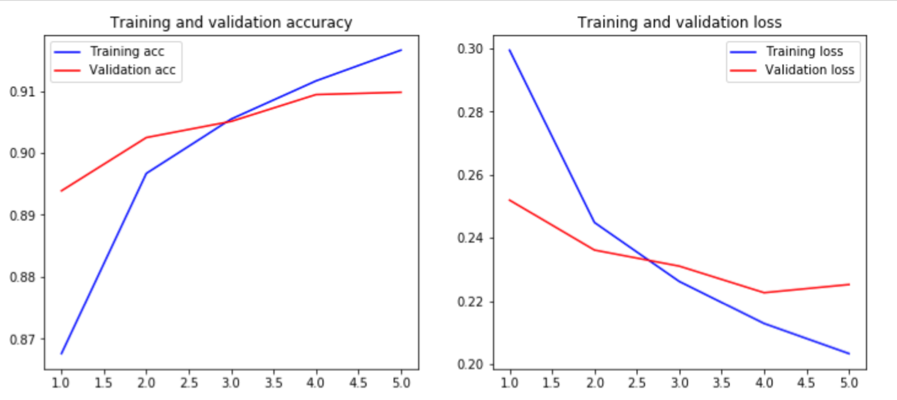
\includegraphics[width=\linewidth]{LSTM400.png}
  \caption{LSTM layer with 400 neurons.}
  \label{fig:lstm400}
\end{figure} . 
\item Changing the data split to have more training samples, to be 90\% training data:
\\The result: the accuracy on testing data is 83\% and accuracy on validation data is 89\%. Figure \ref{fig:lstm90}
\begin{figure}[h!]
  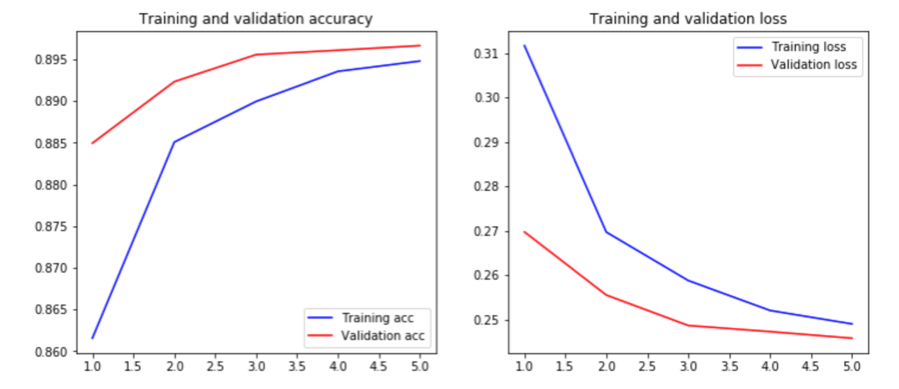
\includegraphics[width=\linewidth]{train90.png}
  \caption{LSTM model with 90\% for training data.}
  \label{fig:lstm90}
\end{figure} . 
\item Change the dictionary for the embedding to include only the testing data without the validation data to simulate the testing data status.
\\ The result:  accuracy on testing data is 83\% and accuracy on validation data is 89\%. Figure \ref{fig:lstmvoc}
\begin{figure}[h!]
  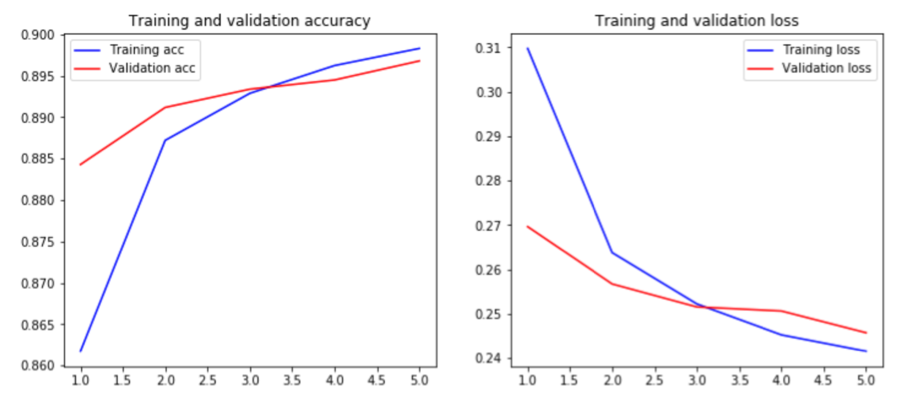
\includegraphics[width=\linewidth]{vocabChange.png}
  \caption{LSTM with embedding dictionary that doesn't have vocabularies from the validation data .}
  \label{fig:lstmvoc}
\end{figure} . 
\end{itemize}

